\documentclass[conference]{IEEEtran}
\usepackage{amssymb}

\newtheorem{mydef}{Definition}

\providecommand{\e}[1]{\ensuremath{\times 10^{#1}}}
\usepackage[normalem]{ulem}
\usepackage[ruled,vlined]{algorithm2e}
\usepackage{epsfig}
\usepackage{subfigure}
\usepackage{tabularx}
\usepackage{graphics}
%\usepackage[pdftex]{graphicx}

\begin{document}

\title{Search of maximal unique matches in multi-core architectures}

\author{\IEEEauthorblockA{Julio C\'esar Garc\'ia Vizca\'ino}
\IEEEauthorblockA{Computer Architecture and Operating Systems,\\\
Campus UAB, Edifici Q,\\
08193 Bellaterra (Barcelona), Spain.\\
Email: juliocesar.garcia@caos.uab.es}
\and
\IEEEauthorblockA{Antonio Espinosa\\
Email: antonio.espinosa@caos.uab.es}
\IEEEauthorblockA{Juan Carlos Moure\\
juancarlos.moure@uab.es}
\and
\IEEEauthorblockA{Porfidio Hern\'andez\\
Email: porfidio.hernandez@uab.es}}

\maketitle

\begin{abstract}
  Maximal Unique Matches are common substrings that match a Reference and a Query genome. They are exact, unique and maximal; that is, they cannot be extended in left or right direction without incurring a mismatch. The computation of MUMs in large genomes is a heavy and repetitive task, so there is a fair chance to parallelize and execute this search in multi-core architectures. This research uses multi-core architectures to search for MUMs in genomic sequences with a suffix tree. The Reference genome is indexed by using a suffix tree in main memory and then a parallelized algorithm searches for MUMs in Query genome which is read by several threads. We have a near linear speedup according to the number of cores used. This approach is based on MUMmer, a genome alignment tool, which is able to search for Maximal Unique Matches (MUMs). 
\end{abstract}

\begin{IEEEkeywords}
Indexed Search, Bioinformatics, Maximal Unique Match, Multi-core architectures, Parallelization
\end{IEEEkeywords}

\section{Introduction} 
\label{}
Modern sequencing, computational technologies and advances in bioinformatics has made whole genome sequencing possible. One resulting challenge is the fast alignment of whole genomes. Dynamic programming is too slow for aligning two large genomes, hundreds of Mbp. One very successful approach to performing a Whole Genome Alignment is based on identifying "Maximal Unique Matches", like in \cite{Delcher1999}. This heuristic assumes that one expects substrings occurring in two similar genomes. Maximal Unique Matches (MUMs) are almost surely part of a good alignment of the two sequences and so the Whole Genome Alignment problem can be reduced to aligning the sequence in the gaps between the MUMs. The MUM-problem is defined in Definition \ref{problem}.

\begin{mydef}
\label{problem}
Assume we are given two sequences R,Q $\in \Sigma^*$, and a number L $>$ 0. The Maximal Unique Match problem (MUM-problem) is to find all sequences u $\in \Sigma^*$ with: $|u|\geq L$, u occurs exactly once in R and once in Q, and for any character a $\in \Sigma^*$ neither ua nor au occurs both in R and Q.
\end{mydef}

The problem of searching Maximal Unique Matches for a minimum length between a Reference
string and a Query string has been identified in several applications, one of them is MUMmer \cite{Delcher2003}. MUMmer's algorithm can perform searches of Maximal Unique Matches (MUMs)
with the following use of resources: High use of main memory to store the Reference genome and a null use of multi-core architectures.

If the length of Reference and Query genomes are very huge, the amount of operations to perform in the search of MUMs increases, see Table \ref{tbl:operations}.
\begin{table}[htb]
  \begin{small}
    \begin{center}
      \begin{tabular}{lllll}
        Data structure & L [bp] & Search  & Search [s] & Memory\\
        & & operations & & usage [MB]\\
        \hline
        Suffix tree & 20 & 9,87\e{18}  & 169189,4 & 48665,12\\
        \hline
      \end{tabular}
    \end{center}
  \end{small}
  \caption{Search of Maximal Unique Matches between a reference genome (2960,21Mbp) and query genome (2716,96Mbp)}
  \label{tbl:operations}
\end{table}

The use of multi-core architectures could help reduce the execution time to search for Maximal Unique Matches. Figure \ref{algorithm} shows the process of our data-level parallelism technique. In the first phase we construct the suffix tree for Reference genome in a serial way. The second phase splits the query genome in chunks (one chunk per thread) of a fixed size ($chunk\_size=\frac{|Q|}{\#threads}$)  and it performs the search for MUMs in that chunk; for every suffix in the current chunk we use suffix links to have an $O(m)$ search, the list of MUMs found are MUM candidates, a MUM candidate is a MUM which is unique only in the Reference genome but it may not be in Query genome. Phase 3 gets the real MUMs which are unique in the Reference and Query genome from the list of MUM candidates.

\begin{figure}[htb]   
\begin{center} 
  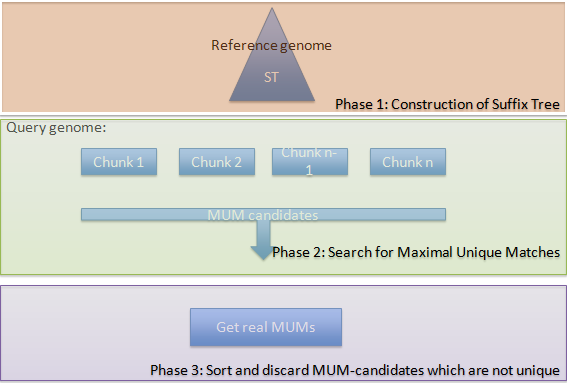
\includegraphics[width=7.5cm,height=5cm]{PhasesST.png}
\end{center} 
\caption{Find MUMs in multi-core architectures for whole genome alignment.} 
\label{algorithm} 
\end{figure} 

The rest of this paper is organized as follows. Section 2 gives some definitions used in this paper. Section 3 discusses the related work. Section 4 explains our implementation of parallelization of search for MUMs. Section 5 shows the implementation details of our technique. Section 6 discusses the results of our parallelization. Section 7 concludes the paper. 
\section{The  MUM: an heuristic approach}
Although a pair of conserved genes rarely contain the same entire sequence, they share a lot of short common substrings and some of them are indeed unique to this pair of genes. For example the following two sequences, R and Q:

\begin{center}
    R=\underline{ac} ga \underline{ctc} a \underline{gctac} t \underline{ggtcagctatt} \underline{acttaccgc}\$\\
    Q=\underline{ac} tt \underline{ctc} t \underline{gctac} \underline{ggtcagctatt} c \underline{acttaccgc}\$\\
\end{center}
    It is clear that sequences R and Q have many common substrings, they are: ac, ctc, gctac, ggtcagctatt, acttaccgc.
    
Among those five common substrings, ac is the only substring that is not unique. It occurs more than once in both sequences. You can also observe that actually a, c, t, and g are common substrings of R and Q. However, they are not maximal, i.e. they are contained in at least one longer common substrings. We are only interested in those that are of maximal length.

Our aim is to search for all these short common substrings. Given genomes R and Q, we need to find all common substrings which are unique and of maximal length. Each of such common substrings is known as Maximum Unique Match (MUM). For almost every conserved gene pairs, there exist at least one MUM which is unique to them.

For example, assuming d = 3, sequences R and Q in the previous example has four MUMs: ctc, gctac, ggtcagctatt, acttaccgc. Substring ac is not an MUM because its length is smaller than the value of d and it is not unique to both sequences.

\begin{center}
    R=\xout{ac} ga \sout{ctc} a \uwave{gctac} t \uuline{ggtcagctatt} \uline{acttaccgc}\$\\
    Q=\xout{ac} tt \sout{ctc} t \uwave{gctac} \uuline{ggtcagctatt} c \uline{acttaccgc}\$\\
\end{center}

The concept of MUM is important in Whole Genome Alignment because a significantly long MUM is very likely to be part of the global alignment.
\subsection{Search for MUMs in a suffix tree} 
The key idea in this method is to build a suffix tree for genome R, a data structure which allows finding, all distinct subsequences in a given genome.

A suffix tree is a data structure which indexes a whole string in every suffix. It allows finding all matches between a Reference genome (suffix tree) and a Query genome. It can also check for unique matches in the Reference very easily just to check if the match ends in a leaf node and by checking the character immediately preceding the start of this match it is possible to determine whether it is a maximal match. To understand the efficient search for matches in a suffix tree, time complexity is $O(m)$ where $m$ is the length of query genome, it is used a suffix link. 

\begin{mydef}
A suffix link points from a source node $s$ in suffix tree to another destination node $d$ in suffix tree if the string label from the root node to node $d$ is equal to the label from root node to $s$ with the first character removed.
\end{mydef}

In Figure \ref{fig:st} is shown the suffix tree, green lines are suffix links and boxes are start position of every suffix. For instance, the string label of node $i$ in Figure \ref{fig:st} is tgt and next suffix $i+1$ is gt. So that is exactly the tree position corresponding to the next position in the Query genome.

\begin{figure}[htb]
  \centering
  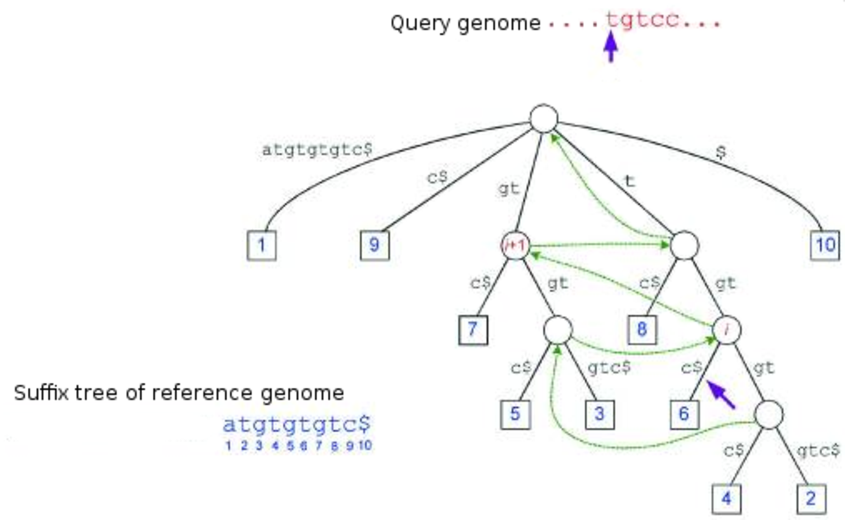
\includegraphics[width=8.5cm,height=5cm]{st-mum.pdf}
  \caption{Suffix tree and its use to find matches between a reference and query genome \cite{Delcher2002}.}
\label{fig:st}
\end{figure}

In Figure \ref{fig:st} the match gtc which starts at $i+1$ in the query genome and node 7 in the suffix tree is not maximal on the left because the preceeding character in both strings is a t.

  By construction, the location of a match in the suffix tree represents a substring of the Reference genome which maximally matches a prefix of \texttt{query suffix}. Thus it is only necessary to verify that, the match is long enough, that it is unique in the Reference genome and that the match is also left maximal. This is done as follows:
\begin{enumerate}
  \item
  Does \texttt{match} represent a substring of length at least \texttt{minimum match length}?
   \item Does \texttt{match} correspond to a leaf edge? Then  then the string represented by the match is unique in the Reference genome.
  \item Is the match left maximal? This is true if one of the following conditions hold:
  \begin{itemize}
  \item   
  The suffix of the query currently considered is the first suffix, or 
  \item 
  The string represented by \texttt{match} is a prefix of the Reference genome,  or
  \item  
  The characters immediately to the left of the matching strings in the Reference genome and the query sequence are different.
  \end{itemize}
  \end{enumerate}
  If all conditions 1-3 are true, then this MUM is stored in a list of MUM-candidates as it is shown in Figure \ref{candidates}. If a match is found but it doesn't reach a leaf node then this match is dropped as it is shown in Figure \ref{candidates}. A MUM-candidate is saved in an array of type MUM-candidate which has the following information:
Position in Reference genome, Position in Query genome and Length of match.

 \begin{figure}[htb]  
 \begin{center} 
  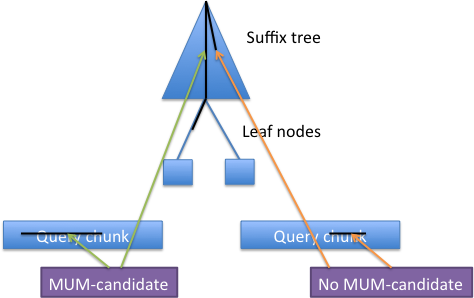
\includegraphics[width=6.5cm,height=4cm]{MUM-candidates.png}
 \end{center} 
 \caption{Finding MUMs in a suffix tree. Blue box represents a leaf node and it saves the start position of its suffix.} 
 \label{candidates} 
 \end{figure}  
 
 The current serial search method is summarized in Algorithm \ref{alg:find}, the first suffix is \textbf{always} searched from the root node in Suffix Tree and rest of suffixes are searched with suffix links from the node in suffix tree from previous search, this algorithm has an $O(m)$ complexity.
\begin{algorithm}[htb]
  \label{alg:find}
  \SetKwInOut{Input}{input}
  \SetKwInOut{Output}{output}
  \SetKwData{R}{R}
  \SetKwData{Q}{Q}
  \SetKwData{ST}{ST}
  \SetKwData{Len}{L}
  \SetKwFunction{Length}{length}
  \SetKwData{Leaf}{leaf}
  \SetKwData{MUMs}{MUMs}
  \SetKwData{MUMcands}{MUMcands}
  \SetKwData{loc}{loc}
  \SetKwFunction{buildST}{buildST}
  \SetKwFunction{TraverseSuffixTree}{TraverseSuffixTree}
  \SetKwFunction{suflink}{suffixlink}
  \SetKwFunction{isRootNode}{isRootNode}
  \SetKwFunction{isLeafNode}{isLeafNode}
  \SetKwFunction{saveMUMcand}{saveMUMcand}
  \SetKwFunction{cleanMUMcand}{cleanMUMcand}
  \Input{\R, \Q, \Len}
  \Output{List of \MUMs of \Length$\geq$ \Len, with start position in \R and \Q and \Length}
  \Begin{
  \ST$\leftarrow$ \buildST{\R}\;
  \loc$\leftarrow$ \TraverseSuffixTree{$\Q[0]$,ROOT,\ST}\;
  \For{i=1 to $|Q|$}{
    \If{\isLeafNode{\loc} and \loc.length $\ge$ \Len }{
    \tcc{Leaf saves the position of a suffix in ST.}\;
        \If{$\R[\Leaf-1]\neq \Q[i-1]$}{
            \MUMcands$\leftarrow$ \saveMUMcand{$\R_{\Leaf}$,$i$,\Length}\;
        }
    }
  \eIf{\isRootNode{loc}}{
  \loc$\leftarrow$ \TraverseSuffixTree{$\Q[i+1]$,ROOT,\ST}\;
  }{
  \suflink{\ST,\loc}\;
  \loc$\leftarrow$ \TraverseSuffixTree{$\Q[i+1]$,\loc.node,\ST}\;
  }
  }
  \tcc{Get unique MUMs from list of MUM-candidates.}\;
  \MUMs$\leftarrow$ \cleanMUMcand{\MUMcands}
  }
  \caption{Search for MUMs in a suffix tree.}
\end{algorithm}
 MUMs can cover 100\% of the known  conserved gene pairs. Moreover, finding all MUMs  can be done in almost linear time because of the use of suffix links, without this artifact we should start every traversal in Suffix Tree from root node adding more execution time because we scan a longer string. Since a Suffix Tree can be queried several times, it is very likely to have more than one query  at the same time. So far, Algorithm \ref{alg:find} is a serial execution because it does not check for more than one suffix at the same time.
 
This problem is a very high intensive computing task, for every substring in the query genome the search for a Maximum Unique Match has to be performed.
\section{Related work}
Search for Maximal Unique Matches to do Whole Genome Alignment was proposed in \cite{Delcher1999}. There have been some previous work in the parallelization to search for matches in genomic data, like \cite{OguzhanKulekci2011,Mongelli,Kouzinopoulos2005}, however these works are focused in fixed patterns and read alignment. On the other hand, there have been achievements in parallelization of Whole genome alignment like \cite{Meng2005}. The parallelization of searching MUMs with a suffix tree is research field not covered very deep. In \cite{Encarnac2011} is explained the use of threads to search for MUMs but without access to source code to check their implementation; and in \cite{Schatz2007} there is an approach similar to this work, however, it is more focused with GPU and CPU hybrid architectures. Our approach is based on the use of multi-core architectures with OpenMP and Suffix Tree to search for MUMs.
\section{Parallel algorithm}  
The sequential version of the MUM search between a Reference and Query genome trades high computation time when executed in a single machine. Suffix tree is the archetypical index structure used in bioinformatics. For large-scale bioinformatics applications, however, memory consumption and memory bandwidth really becomes a bottleneck. Moreover, the algorithm to search for MUMs involves comparing the search for a character to the character stored at a specific node at every level of the tree, and traversing a child node based on the comparison results. Only one node at each level is actually accessed for every traversal in Suffix Tree, resulting in ineffective cache line utilization, Pre-fetching techniques are not suitable since the result of the comparison in previous node is required before loading the appropriate child node. Moreover, meanwhile the Algorithm \ref{alg:find} shows a $O(m)$ complexity by using suffix links, this feature has the disadvantage of a quite random access to the next node used to traverse the suffix tree. Traversing the suffix tree involves following a set of pointers to different memory regions. As a consequence a search for MUM typically involves a long-latency TLB/cache miss at each level of the tree, leading to ineffective utilization of the processor resources. To hide this long latency we propose to use multi-core architectures.

Previously the algorithm for sequence alignment was described in detail. Now our own proposal of a parallelization of MUM search within multi-core architecture is explained.

There are two resources to improve in this algorithm: Memory usage and CPU. The former was generally improved because it allows being executed in architectures where there is no memory restriction and suffix tree allows searching more than one suffix at the same time. To improve the performance of the algorithm a data-level parallelism technique is deployed in advance to genome alignment.

Our technique is divided in three phases following:
\begin{enumerate}
\item Splitting query genome data (chunks) according to the number of available cores using 1 thread per core. Chunk size is computed with the total of threads used, thus the chunk size is fixed.
\item Parallel execution of the task of Algorithm \ref{alg:find} for every chunk, after finishing its task every thread has its own list of MUM-candidates.
\item Get the final list of MUMs from every MUM-candidate list of all threads.
\end{enumerate}
The main idea behind using a Maximal Unique Match (MUM): it is possible to cover a huge region of a genome when reference and query genomes are very closely related. However, to get a MUM  requires an important feature its uniqueness. Uniqueness can only be found when a whole genome is checked, see Figure \ref{Whole-MUM}. If some part of it is only evaluated we could miss the rest of the genome. In other words, after finding MUMs within a chunk it is not possible to determine if the MUM found is or not a "unique" MUM, globally in the query genome,  because these MUMs are unique only in the chunk that has been read, the rest of the genome it is not known until all query genome has been read. In Figure \ref{Whole-MUM} is shown the consequences of using chunks for query genome. Meanwhile we may speed up the MUM search we need to deal with the discard of MUM-candidates which are not a real MUM. So that, after finding all MUM-candidates for every thread we need to verify which of MUM-candidates are MUM.

\begin{figure}[htb]  
\begin{center} 
  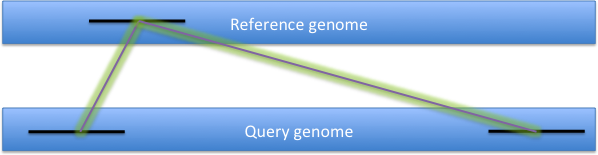
\includegraphics[width=6cm,height=3cm]{Whole-MUM.png}
\end{center} 
\caption{MUM in reference genome but not in query genome.} 
\label{Whole-MUM} 
\end{figure}

In Figure \ref{algorithm} we can see phase 3 which involves to extract the list of MUM from the set of MUM-candidates of every chunk in the query genome. In order to get the real MUMs we filter MUM-candidates that are overlapped by bigger MUM-candidates.
\section{Implementation} 
\label{implementation}
\subsection*{Split query genome}  
As it was previously explained, the approach is to use a fixed size division of query genome. To split query genome the algorithm needs to know in advance how many chunks will be used. Then every chunk is computed with two pointers (left and right end) which points out query genome in main memory.
\subsection*{Finding MUMs}
The parallelization is carried out with OpenMP, the Algorithm \ref{alg:find} is applied for every chunk. The algorithm to search MUMs is a process which can be executed without any data dependency. 

Firstly, from Algorithm \ref{alg:find} some variables are shared among the threads in our OpenMP implementation: Suffix Tree, Reference genome and Query genome. Secondly, some variables are private for every thread: the location pointer to Suffix Tree, the pointer to the chunk of Query genome assigned to each thread and the array of MUM-candidate type.

However, when we split a query sequence the following problems arise.
\subsubsection*{Chunk size}
Chunk size is a performance factor because we need to have an ideal size to have balanced workload among threads. Since we can not know in advance which region in the Query genome has more MUMs, it is very likely that some threads may finish before. 
\subsubsection*{Different MUM-candidate in Query genome}
Additional MUMs can be found because we can not know if the MUM-candidate is unique or not. In other words, to stream the Query genome with only one thread gives the correct list of MUM-candidates, when we split the Query genome, every chunk may have additional MUM-candidates that could be avoided by reading the whole Query genome. These additional MUM-candidates are an overhead in phase 2 and 3 of our implementation in Figure \ref{algorithm}.

The total number of iterations is the number of chunks created. Every iteration means the whole search of MUMs within a chunk, following the Algorithm \ref{alg:find}, if the right end of chunk is not the end of the query sequence and there are still nucleotides to match then traversal of suffix tree until it occurs a mismatch or a MUM-candidate is found or it reaches the end of Query genome.

The key factors in this phase are: number of chunks (every chunk is private for each thread), size of chunks (delimiters for chunks are private for each thread) and number of threads.
\subsection*{Get real MUMs}
This phase is applied with an algorithm for the set of MUM-candidates. These are ordered with quicksort according to position in Query genome. Every thread has found a set of MUM-candidates from previous phase but all threads don't produce the MUM-candidates in order. Thus a quicksort is required.

After quicksort we need to get the real MUMs. A real MUM is unique in the whole reference and query genome. Those MUM-candidates which are overlapped by bigger MUMs are discarded too, see Figure \ref{real-mums}.
\begin{figure}[htb]  
\begin{center} 
  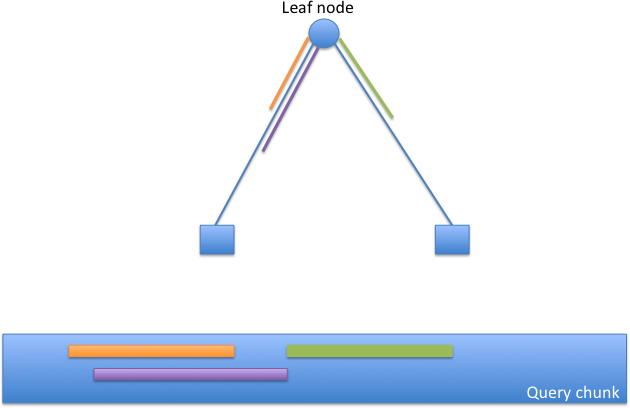
\includegraphics[width=5cm,height=3cm]{MUMs.png}
  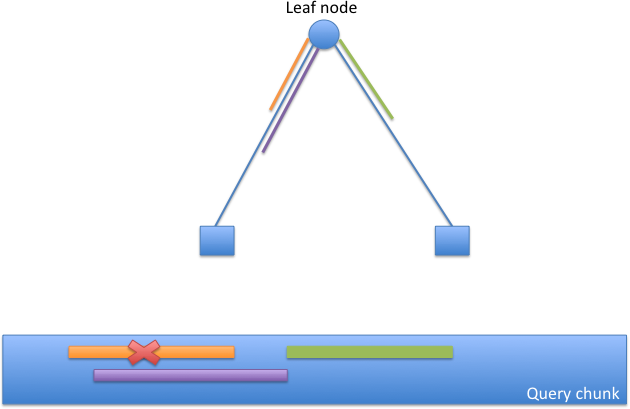
\includegraphics[width=5cm,height=3cm]{Remove-MUMs.png}
\end{center} 
\caption{Getting Real MUMs. MUM-candidate in orange colour is discarded because another MUM-candidate has a larger length and they have same match in leaf of the Suffix Tree.} 
\label{real-mums} 
\end{figure}
The final output has the following format:
\begin{verbatim} 
>Information about the query sequence
Position_in_R Position_in_Q Length_of_MUM
\end{verbatim}
\section{Experiments and results}
To verify that our approach, can have a better performance to search for MUMs between a Query and Reference genome, we check that output of MUMmer and our approach has the same MUMs. This test was carried out in the following node:
\begin{itemize}
\item Hardware:  
\begin{itemize}
\item 2 Processor Intel(R) Xeon(R) E5645 @ 2.4GHz of 6 cores each one, 32KB L1 cache, 256KB L2 and 12MB L3 shared cache per socket.
\item RAM: 96 GB
\end{itemize} 
\item  Software: 
\begin{itemize}
\item Linux Kernel 2.6.32-220.el6.x86\_64 \#1 SMP
\item gcc 4.7.0 with OpenMP support
\end{itemize}  
\item Genomes:
  \begin{itemize}
    \item Reference: Silkworm genome, 487.6 [Mbp]
    \item Query: Red imported fire ant genome, 335.7 [Mbp]
  \end{itemize}
\end{itemize}
The main objective of the test was to check the performance to search for MUMs in multi-core architectures by using OpenMP (threads). The variables to control were: number of chunks for query genome, number of threads: 1, 6, 12 and 24 threads with affinity and OpenMP scheduling: static with chunk size of 1.

The times were collected only for the parallel region of OpenMP. This parallel region is the algorithm to search MUMs.

One key aspect of the test deployed was to assure the execution of every thread in a single core, that is no other thread is competing for the same cache. Affinity is a requirement because we need to ensure the scalability of our proposal, without affinity even a number of threads below the number of cores might be in the same core. Affinity ensures us a proper use of performance in a multi-core architecture.

The construction of the suffix tree for the reference genome of length 487.6 [Mbp] takes 208.71 [s] to build and it uses 10.12[GB] of memory. The minimum length for a MUM was 20 [bp]. The query sequence of length 335.7 [Mbp] was divided in chunks equal to the available threads.

Times were collected during the execution of the experiments: execution time to search for MUMs in parallel region with the function omp\_get\_wtime of OpenMP.

Figure \ref{fig:speedup} shows the speedup for our parallelization to search for MUMs. Moreover, from this Figure \ref{fig:speedup} we can conclude that we got a near linear speedup with 12 threads, which is the maximum number of cores. Then there is a reduction in the linear speedup because we start using more than 1 thread per core and this causes a degradation in the phase of searching MUMs. As we can see in Figure \ref{fig:speedup} the better speedup is with one thread per core and it is a consequence of similarity between our reference and query genome.

\begin{figure}[htb]
  \centering
  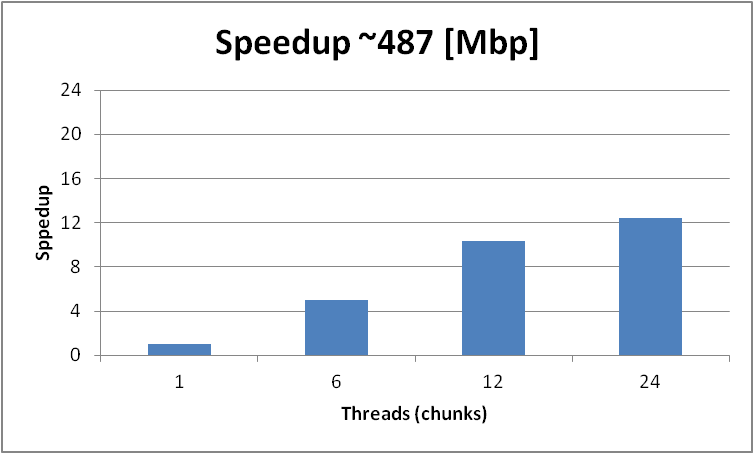
\includegraphics[width=8.5cm,height=5cm]{speedup-big.png}
  \caption{Speedup of our approach to search MUMs in multi-core architectures with OpenMP.}
  \label{fig:speedup}
 \end{figure}  
 
Our goal is to get the best performance of a multicore architecture while searching MUMs and from the Figure \ref{fig:time} we can watch a decent performance up to 12 threads, when there is more than one thread per core (Hyper-threading) the search time is not reduced, see Figure \ref{fig:time}.

\begin{figure}[htb]
  \centering
  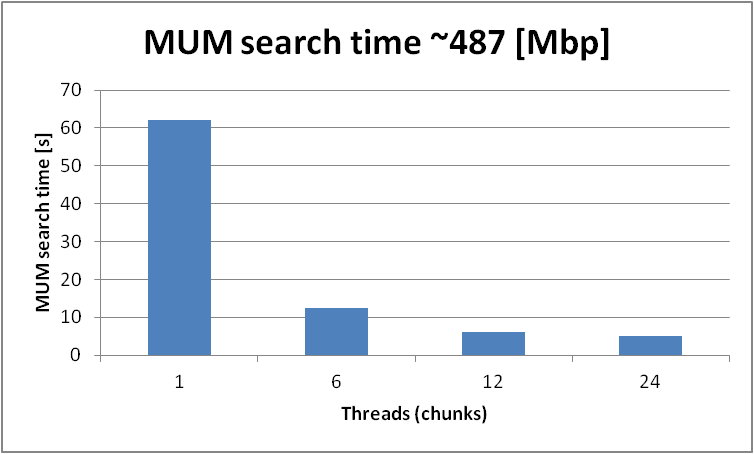
\includegraphics[width=8.5cm,height=5cm]{time.png}
  \caption{Search for MUMs time of our approach in multi-core architectures with OpenMP.}
  \label{fig:time}
 \end{figure}  

The reason of this behavior is because the traversal of a huge suffix tree makes the search of MUMs a high intensive memory bound problem. So that the processor is waiting for the next portion of data to traverse the suffix tree. Our Suffix Tree is implemented by using linked list. The linked list have items in disjoint areas of memory. To traverse the list the cache lines cannot be utilized effectively. One could say that the linked list is cache line hostile, or that the linked list maximizes cache line misses. The disjoint memory will make traversing of the linked list slow because RAM fetching will be used extensively. This layout of our suffix tree and the random search of MUMs do not help to a better use of processor resources. The use of suffix links reduces the time complexity to search for a MUM in a suffix tree but it is not very cache-friendly. The speedup in Figure \ref{fig:speedup} with one thread per core is because we take advantage of the memory heriarchy of cache level 1 and 2. However, there is space to reduce the execution time in phase 2 and 3 of our approach by using a better effective  memory bandwidth. 

To improve the performance of our approach the following proposals may be used:
\begin{itemize}
  \item Prefetching: this may work because we know in advance what information from suffix tree and query sequence we need in every traversal of suffix tree. If we can allow the use of some part of suffix tree be stored and read in cache by several threads which request that substree. However, because we use suffix links to jump to another part of suffix tree so that a new part of suffix tree would have to be read.
  \item Explicit cache management: this is a obvious consequence of previous bullet because we may need to store part of the suffix tree in some cache-level of processor.
  \item An improved traversal of suffix tree would improve the overall performance of search of MUMs. So far, one thread traverses the suffix tree if we add multithread traversal of suffix tree to find next edge in the match path we would reduce the execution time.
\end{itemize}
%% \appendix

\section{Conclusions}
This paper presents an evaluation of performance to search MUMs of a query and reference genome in multi-core architectures with OpenMP. The search of MUMs is performed in a suffix tree and the list of MUMs can help in the process of whole genome alignment. The results shows that the heaviest section of searching MUMs in a suffix tree is improved with the use of a multi-core architecture. Although we got a near linear speedup with only one thread per core, there are more improvements to do. These improvements involve a better use of resources (memory and CPU) when we have more than thread per core. In spite of suffix tree is a good data structure for string matching, when is used in multi-core architectures it shows a poor performance in terms of effective memory bandwidth to search MUMs.

From the results obtained we conclude that bottleneck is in our data structure: suffix tree. We require to handle a strategy to traverse a suffix tree in multi-core architectures, this approach only queries the suffix tree for one string at a time. However, the traversal of suffix tree is still done in a serial way.
%% \label{}

\section*{Acknowledgements}
This work was supported by grant from ``Ejecuci\'on eficiente de aplicaciones multidisciplinares: nuevos desaf\'ios en la era multi/many core, with reference TIN2011-28689-C02-01''.
%% References
%%
%% Following citation commands can be used in the body text:
%% Usage of \cite is as follows:
%%   \cite{key}         ==>>  [#]
%%   \cite[chap. 2]{key} ==>> [#, chap. 2]
%%

%% References with BibTeX database:
\section*{References}
\bibliographystyle{IEEEtran}
\bibliography{mum-multithread}

\end{document}

%%
%% End of file `procs-template.tex'. 